\documentclass[10pt,red]{beamer} 
% change the alerted colour to blue
\setbeamercolor{alerted text}{fg=blue}

\usetheme{berlin}
% theme split
\usepackage{beamerthemesplit}

\usepackage{booktabs,array,}
\usepackage{listings}
\usepackage{hyperref}
\usepackage{verbatim,moreverb}
\usepackage{tikz}

\usepackage{color}

\definecolor{dkgreen}{rgb}{0,0.6,0}
\definecolor{gray}{rgb}{0.5,0.5,0.5}
\definecolor{mauve}{rgb}{0.58,0,0.82}

\lstset{frame=tb,
  language = Java,
  aboveskip=3mm,
  belowskip=3mm,
  showstringspaces=true,
  columns=flexible,
  basicstyle={\small\ttfamily},
  numbers=none,
  numberstyle=\tiny\color{gray},
  keywordstyle=\color{blue},
  commentstyle=\color{dkgreen},
  stringstyle=\color{mauve},
  breaklines=true,
  breakatwhitespace=true
  tabsize=4
}
% theme shadow
\usepackage{beamerthemeshadow}

% For including figures
\usepackage{graphicx}

% logo
\logo{
\includegraphics[height=1cm]{iitblogo.pdf}}


% sf family, bold font
\sffamily \bfseries
% Beginning of title page
\title
% content inside [] appears at bottom of all page. content inside {} appears on first page as title. double backslash means line change 
[
	Raspberry Pi Hardware Development	% bottom
	\hspace{0.5cm}
	\insertframenumber/\inserttotalframenumber
]
{
	External interrupt on RPi using threading concept.
}

\author
[
	www.e-yantra.org
]
{
	e-Yantra Team \\
  Embedded Real-Time Systems Lab\\
  Indian Institute of Technology-Bombay \\
}
\date
{
IIT Bombay \\ {\today}
}
 
 
\begin{document} 

% Slide-1: Title Page
\begin{frame}
	\titlepage
\end{frame} 
\section{Interrupt}
\begin{frame}
	\frametitle{What is Interrupt} \pause
		\begin{enumerate}[$\checkmark$]
			\item<+-|alert@+> Any signal that causes break in continuity of some ongoing process. \\[10pt]
			\item<+-|alert@+> While main program is running, if an interrupt occurs, execution of main program is stopped, and program counter goes to address of ISR. \\[10pt]  
			\item<+-|alert@+> Interrupt Service Routine: Program that needs to be executed when interrupt occurs. \\[10pt]
			\item<+-|alert@+> After program inside ISR is executed completely, program counter returns back to point where main program was interrupted. \\[10pt]
		\end{enumerate}  
\end{frame}
\begin{frame}
	\frametitle{Threading in Python} \pause
	\begin{enumerate}[$\checkmark$]
		\item<+-|alert@+> Running several threads is similar to running many program concurrently.
		\item<+-|alert@+>But it has some advantages i.e. it access the same data space.
	\end{enumerate}
\end{frame}
\section{Experiment}
\begin{frame}
	\frametitle{Experiment}
	\textbf{Switch Interrupt on Raspberry Pi using threading.}
\end{frame}
\begin{frame}
	\frametitle{Hardware Required for the experiments:}
	\begin{tabular}{c c c c}
		 1.  & Breadboard & & 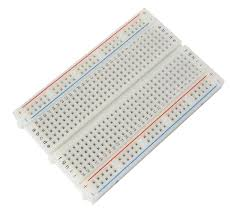
\includegraphics[scale = 0.2]{breadboard} \\ \pause
		 2.  & Switch	& &	
\includegraphics[scale = 0.1]{push_button} \\ \pause
		 3.  & LED (Two Nos.)		&  &	
\includegraphics[scale = 0.2]{led} \\  \pause
		 4.  & 330 ohm resistor (Two Nos.) & &
\includegraphics[scale = 0.1]{resistor}  \\
	\end{tabular}
\end{frame}
\begin{frame}
	\frametitle{Connection Diagram} \pause
	\centering
	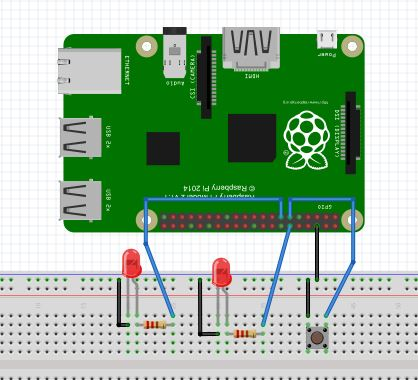
\includegraphics[scale=0.6]{external_interrupt}
\end{frame}
\subsection{Problem Statement}
\begin{frame}
	\frametitle{Problem Statement} \pause
	\textbf{Interfacing two leds with raspberry pi. One led will blink continuously. Another led will glow for 1 second when switch is pressed.}
\end{frame}
\begin{frame}
	\hskip4cm
	\textbf{\LARGE Thank You!} \\[20pt]
	\hskip3cm
	\scriptsize Post your queries on: 
	\hyperref[www.e-yantra.org]{\color{blue} http://qa.e-yantra.org/ \color{black}} 
\end{frame}
\end{document} 

\end{document}